%!TEX root = presentazionelancia.tex
\setlength{\parskip}{\baselineskip} 
\section*{Introduction}
\begin{frame}[t]
\frametitle{Introduction}
What is TAO?

\begin{block}{Tao}
	is a geographically distribute store
	\begin{itemize}
		\item deployed at Facebook
	 	\item with efficient and timely access to social graph
	 	\item using a fixed set of query
	 	\item replacing memcache
	 	\item running on thousands of machines
	 	\item provide access to many PB of data
	 	\item process a billion reads ad millions of writes each second!
	 \end{itemize} 
\end{block}
\end{frame}

\begin{frame}
\frametitle{The social graph}
Facebook has more than 1 billion active user 
\begin{itemize}
	\item recording relationships,
	\item sharing interests,
	\item uploading pictures and \dots
\end{itemize}

The user experience of Fb comes from rapid, efficient and scalable access to the \emph{social graph}
\end{frame}

\begin{frame}
\begin{columns}
	\begin{column}{0.3\textwidth}
	What's behind an entry in yours Fb page?
	\\~\\
		A single Fb page aggregate and filter hundreds of items from the social graph.
		\\~\\
		producing user-tailored content and checking for privacy %
	\end{column}%
	\begin{column}{0.6\textwidth}%
		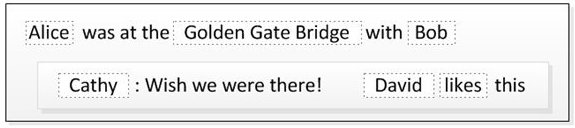
\includegraphics[width=\columnwidth]{social.jpg}%
	\end{column}%
\end{columns}%
\end{frame}%

